\section{Computador} 
Construir um computador parece uma tarefa complicada e assustadora. Porem, uma CPU\footnote{CPU é a sigla para Central Process Unit, ou Unidade Central de Processamento. É o principal item de hardware do computador, que também é conhecido como processador, essa é a parte responsável por calcular e realizar tarefas determinadas pelo usuário.} é bastante simples em operação depois que os fundamentos por trás de todos os seus processos são compreendidos. Este cápitulo destina-se a executar o passo a passo para que qualquer pessoa interessada seja capaz em construir seu próprio computador e obter o conhecimento que acompanha o processo.

\subsection{Modulos}
Para facilitar o compreendimento, e também o desenvolvimento do computador, este capitulo será dividido em alguns subcapitulos, assim cada um abordará uma parte do computador. 

\subsubsection{Clock}
O clock do computador é uma parte essencial para o seu funcionamento. Este tem a função de sincronizar todas as operações. A ação mais rápida que o computador consegue executar é equivalente a uma vibração do seu clock.
\begin{figure}[H] \centering 
  \makebox[\textwidth][c]{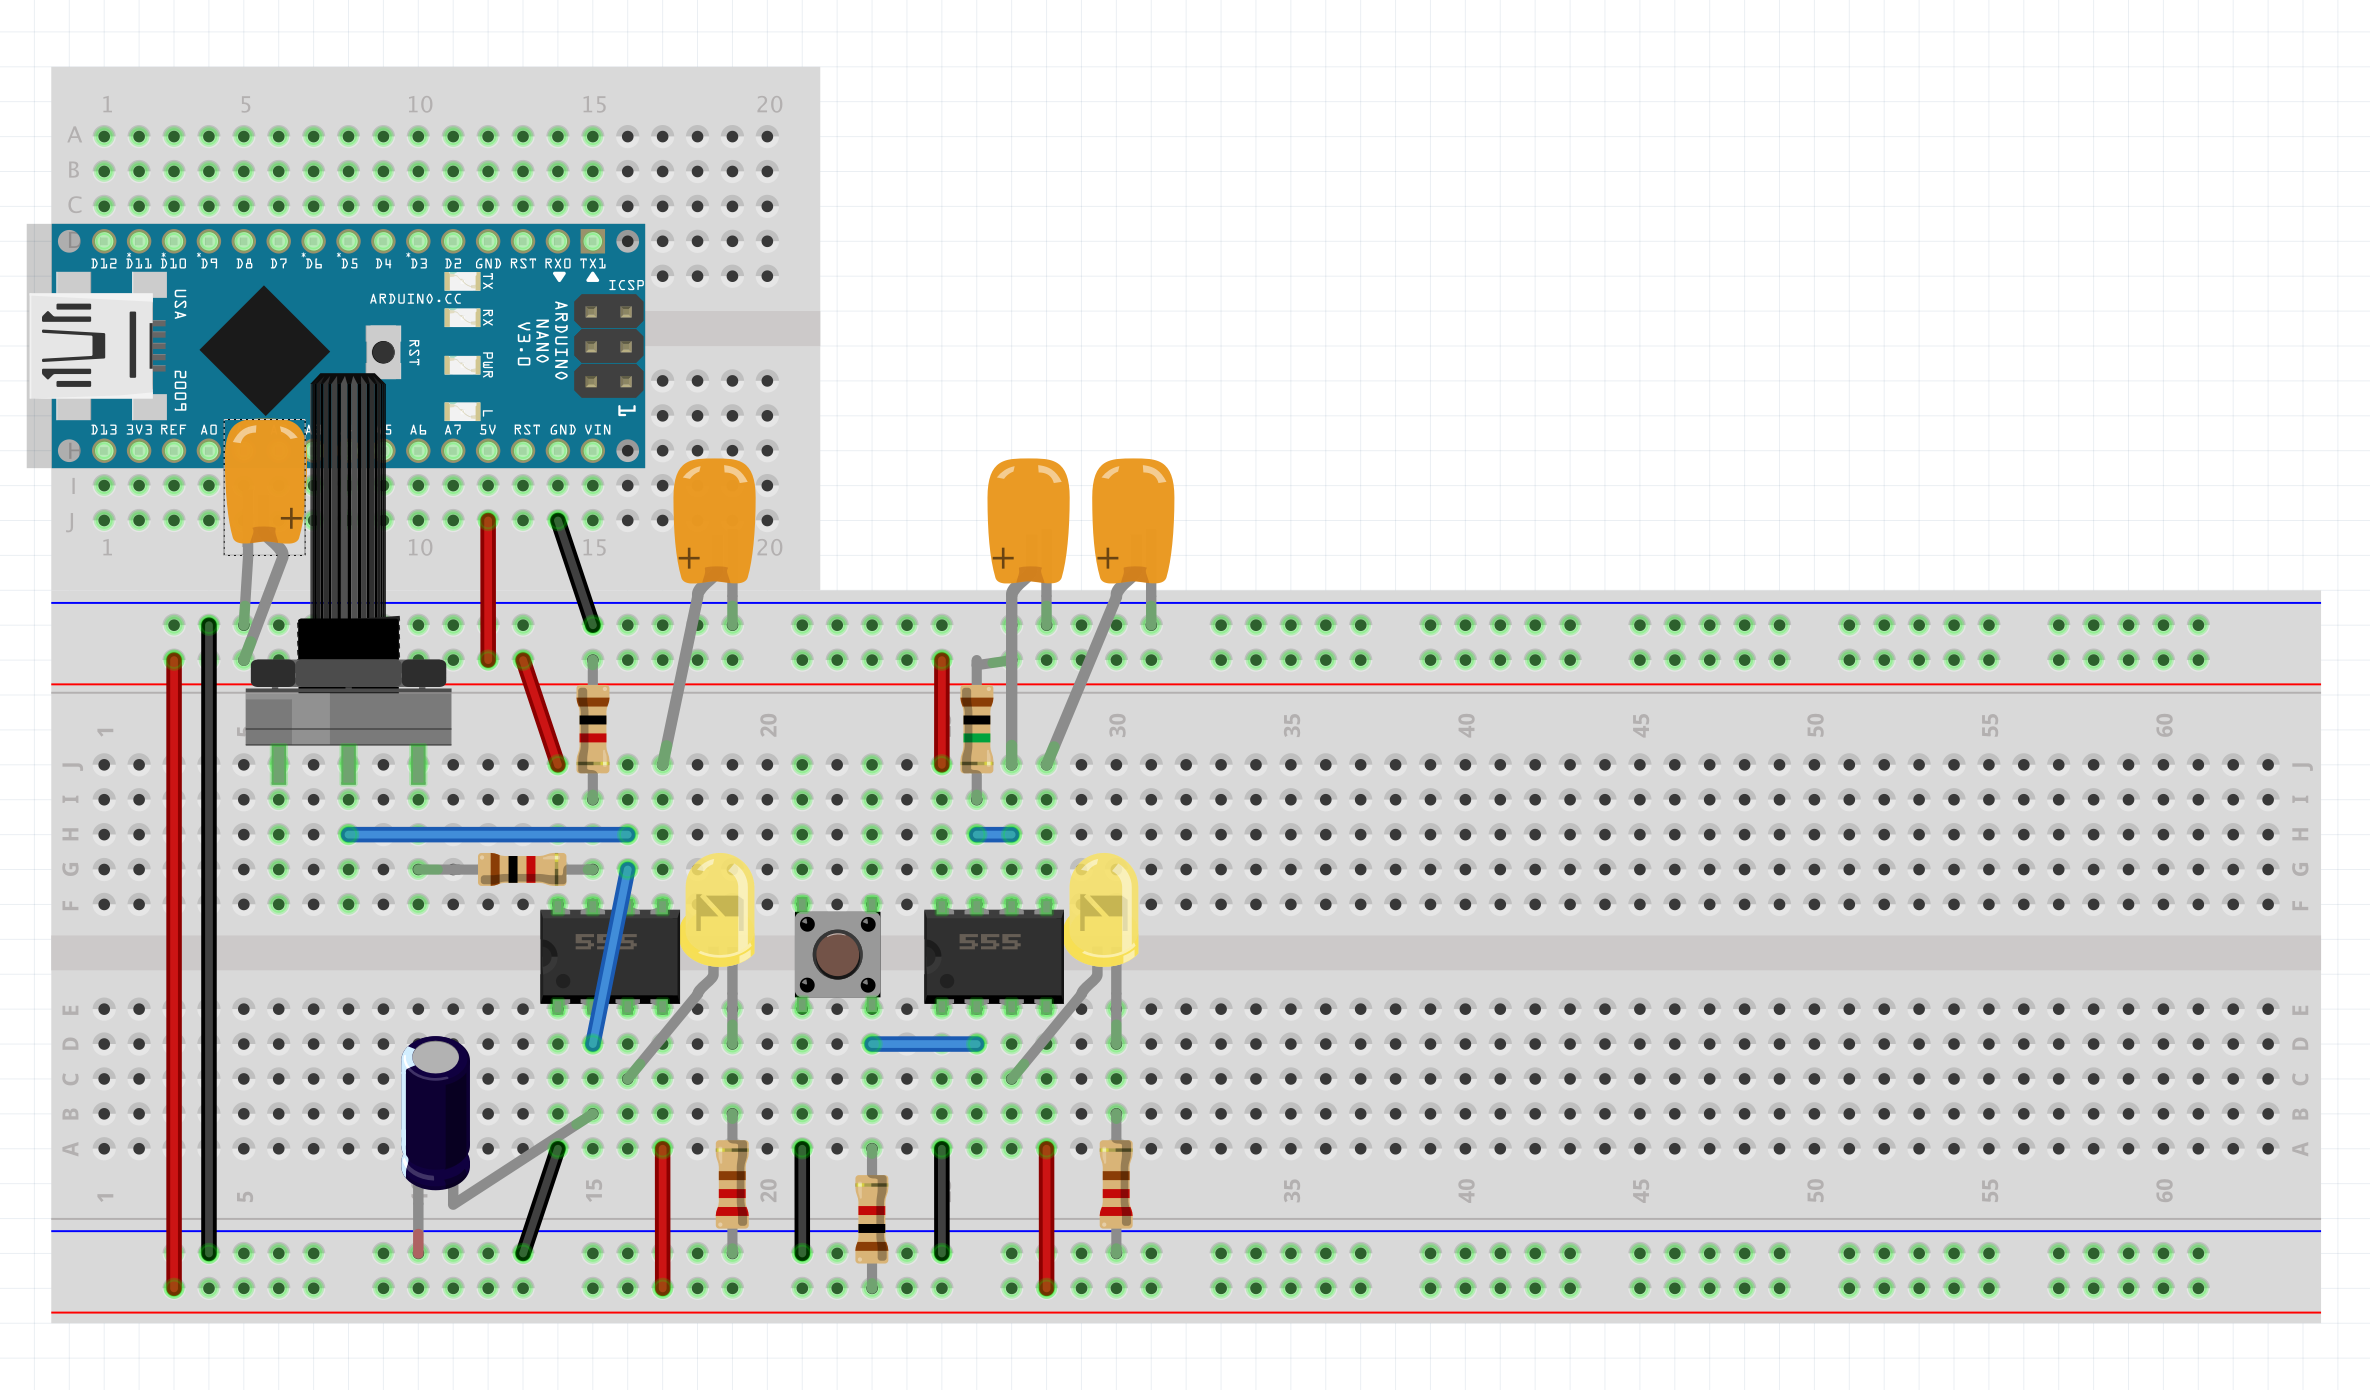
\includegraphics[width=0.8\textwidth]{clock}}
  \caption{\label{fig:1} Esquema do Clock} 
\end{figure}

\subsubsection{Registers}
A maioria das CPUs possuem vários registradores que armazenam pequenas quantidades de dados que a CPU está processando. Em nossa CPU de breadboard, criaremos três registradores de 8 bits: A, B e IR. Os registradores A e B são registradores de uso geral. O IR (instruction register) funciona da mesma forma, porém apenas o usamos para armazenar a instrução atual que está sendo executada.

\subsubsection{Arithmetic logic unit (ALU)}
A parte da unidade lógica aritmética (ALU) de uma CPU geralmente é capaz de executar várias operações aritméticas, bit a bit e de comparação em números binários. Em nossa CPU de breadboard, a ALU pode apenas adicionar e subtrair. Ele está conectado aos registros A e B e gera a soma de A + B ou a diferença de A-B.

\subsubsection{Random access memory (RAM)}
A memória de acesso aleatório (RAM) armazena o programa que o computador está executando, bem como todos os dados que o programa precisa. Nosso computador de breadboard utiliza endereços de 4 bits, o que significa que ele terá apenas 16 bytes de RAM, limitando o tamanho e a complexidade dos programas que ele pode executar.

\subsubsection{Program counter}
O contador do programa (Program counter) conta em binário para acompanhar qual instrução o computador está executando no momento.

\subsubsection{Output register}
O registro de saída é semelhante a qualquer outro registro (como os registros A e B), exceto que, em vez de exibir seu conteúdo em binário em 8 LEDs, ele exibe seu conteúdo em decimal em um display de 7 segmentos. Fazer isso requer alguma lógica complexa.

\subsubsection{CPU control logic}
A lógica de controle é o coração da CPU. É o que define os códigos de operação (opcode) que o processador reconhece e o que acontece quando ele executa cada instrução.

\subsubsection{Materiais Necessários}

\newpage